\newpage

\section{Appendice A: Séries de Taylor et Maclaurin}

\begin{definitionbox}[Séries de Taylor et Maclaurin]
Si une fonction $f$ est indéfiniment dérivable au voisinage d'un point $a$, sa \textbf{série de Taylor} centrée en $a$ est définie par :
$$ f(x) = \sum_{k=0}^{\infty} \frac{f^{(k)}(a)}{k!} (x-a)^k $$
où $f^{(k)}(a)$ est la $k$-ième dérivée de $f$ évaluée en $a$.
\newline
\newline
Dans le cas particulier où $\mathbf{a=0}$, la série est appelée une \textbf{série de Maclaurin}. C'est la forme la plus courante, car elle approxime les fonctions autour de l'origine.
\end{definitionbox}

\subsection{Construction pas à pas d'une série de Taylor}

\begin{intuitionbox}[La logique de la correspondance des dérivées]
L'objectif fondamental d'une série de Taylor est de construire un polynôme, $P(x)$, qui soit une "copie conforme" d'une fonction $f(x)$ autour d'un point $a$. Pour ce faire, on force le polynôme à avoir exactement les mêmes propriétés locales que la fonction : même valeur, même pente, même courbure, etc. Cela se traduit mathématiquement par une exigence : \textbf{la n-ième dérivée du polynôme en $a$ doit être égale à la n-ième dérivée de la fonction en $a$}, et ce pour tous les ordres $n$.

Prenons l'exemple de $f(x) = e^x$ et construisons sa série de Maclaurin (centrée en $a=0$), où $f^{(k)}(0)=1$ pour tout $k$.

\begin{enumerate}
    \item \textbf{Ordre 0 : Faire correspondre la valeur}
    \newline
    \textbf{Objectif :} Le polynôme $P_0(x)$ doit avoir la même valeur que $f(x)$ en $x=0$. On veut $P_0(0) = f(0)$.
    \newline
    \textbf{Solution :} On choisit le polynôme le plus simple, une constante : $P_0(x) = f(0)$. Pour $e^x$, $f(0)=1$, donc $\mathbf{P_0(x) = 1}$.
    \newline
    \textbf{Vérification :} $P_0(0) = 1$. L'objectif est atteint.

    \item \textbf{Ordre 1 : Faire correspondre la première dérivée}
    \newline
    \textbf{Objectif :} On veut un nouveau polynôme $P_1(x)$ qui préserve la correspondance précédente ($P_1(0) = f(0)$) ET qui a la même pente, c'est-à-dire $P_1'(0) = f'(0)$.
    \newline
    \textbf{Solution :} On ajoute un terme en $x$ à notre polynôme précédent : $P_1(x) = P_0(x) + c_1 x = 1 + c_1 x$.
    \newline
    \textbf{Vérification :}
    \begin{itemize}
        \item $P_1(0) = 1 + c_1(0) = 1$. La valeur correspond toujours, car le nouveau terme s'annule en 0.
        \item On dérive : $P_1'(x) = c_1$. Pour que les pentes correspondent en 0, il faut $P_1'(0) = c_1 = f'(0)$. Comme $f'(0)=1$, on doit choisir $\mathbf{c_1=1}$.
    \end{itemize}
    Notre polynôme est maintenant $\mathbf{P_1(x) = 1+x}$.

    \item \textbf{Ordre 2 : Faire correspondre la deuxième dérivée}
    \newline
    \textbf{Objectif :} On veut $P_2(x)$ tel que $P_2(0)=f(0)$, $P_2'(0)=f'(0)$ ET $P_2''(0)=f''(0)$.
    \newline
    \textbf{Solution :} On ajoute un terme en $x^2$ : $P_2(x) = P_1(x) + c_2 x^2 = 1 + x + c_2 x^2$.
    \newline
    \textbf{Vérification :}
    \begin{itemize}
        \item Les dérivées d'ordre 0 et 1 en $x=0$ ne sont pas affectées, car la dérivée de $c_2x^2$ (soit $2c_2x$) et le terme lui-même s'annulent en 0. Les objectifs précédents sont préservés.
        \item On dérive deux fois : $P_2'(x) = 1 + 2c_2x$ et $P_2''(x) = 2c_2$.
        \item Pour que les courbures correspondent, il faut $P_2''(0) = 2c_2 = f''(0)$. Comme $f''(0)=1$, on doit choisir $\mathbf{c_2 = 1/2}$.
    \end{itemize}
    Notre polynôme est $\mathbf{P_2(x) = 1+x+\frac{1}{2}x^2}$.

    \item \textbf{Le schéma général : L'importance de la factorielle}
    \newline
    Pour faire correspondre la $k$-ième dérivée, on ajoute un terme $c_k x^k$.
    \newline
    Quand on dérive $c_k x^k$ exactement $k$ fois, on obtient $c_k \times k!$.
    \newline
    Toutes les dérivées d'ordre inférieur s'annulent en $x=0$. On doit donc avoir :
    $$ P_k^{(k)}(0) = c_k \cdot k! = f^{(k)}(0) $$
    Cela nous donne la règle pour trouver chaque coefficient :
    $$ c_k = \frac{f^{(k)}(0)}{k!} $$
    C'est précisément le coefficient qui apparaît dans la formule de Taylor, et il est choisi pour cette unique raison : forcer la $k$-ième dérivée du polynôme à correspondre parfaitement à celle de la fonction au point de développement.
\end{enumerate}

\tcblower
\centering
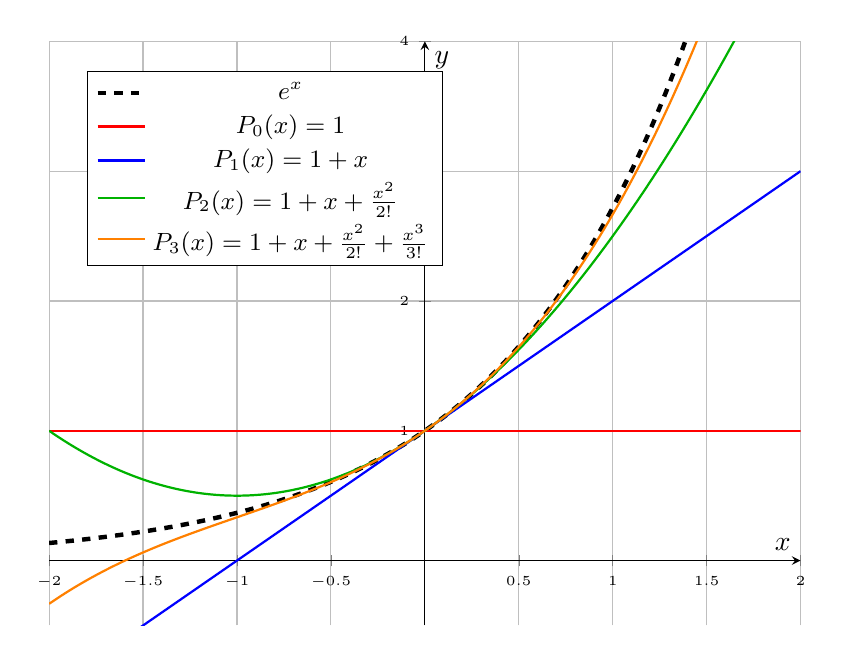
\begin{tikzpicture}
    \begin{axis}[
        xlabel={$x$},
        ylabel={$y$},
        xmin=-2, xmax=2,
        ymin=-0.5, ymax=4,
        axis lines=middle,
        legend style={at={(0.05,0.95)}, anchor=north west, font=\small},
        grid=major,
        samples=150,
        domain=-2:2,
        height=9cm,
        width=\linewidth-1cm,
        tick label style={font=\tiny}
    ]
    
    \addplot[black, dashed, ultra thick] {exp(x)};
    \addlegendentry{$e^x$}

    \addplot[red, thick] {1};
    \addlegendentry{$P_0(x)=1$}

    \addplot[blue, thick] {1+x};
    \addlegendentry{$P_1(x)=1+x$}

    \addplot[green!70!black, thick] {1+x+x^2/2};
    \addlegendentry{$P_2(x)=1+x+\frac{x^2}{2!}$}

    \addplot[orange, thick] {1+x+x^2/2+x^3/6};
    \addlegendentry{$P_3(x)=1+x+\frac{x^2}{2!}+\frac{x^3}{3!}$}

    \end{axis}
\end{tikzpicture}
\par\small\textit{Visualisation de la construction progressive de la série de Maclaurin pour $e^x$.}
\end{intuitionbox}

\subsection{Intuition de la série de Taylor en un point quelconque $a$}

\begin{intuitionbox}[Construire une approximation loin de l'origine]
La série de Maclaurin est puissante, mais elle nous contraint à approximer une fonction uniquement autour de $x=0$. Que faire si l'on s'intéresse au comportement d'une fonction ailleurs, par exemple $f(x)=\ln(x)$ autour de $x=1$ (puisque $\ln(0)$ n'est pas défini) ? C'est là qu'intervient la série de Taylor générale.

L'objectif reste le même : construire un polynôme $P(x)$ qui est une "copie conforme" de $f(x)$ au point $a$. Pour cela, on force les dérivées du polynôme à correspondre à celles de la fonction en ce point $a$. La seule différence est que notre "variable" de base n'est plus $x$, mais l'écart par rapport au centre, c'est-à-dire $(x-a)$.

Prenons l'exemple de $f(x) = \ln(x)$ et construisons sa série centrée en $\mathbf{a=1}$.

\begin{enumerate}
    \item \textbf{Ordre 0 : Faire correspondre la valeur}
    \newline
    \textbf{Objectif :} $P_0(a) = f(a)$.
    \newline
    \textbf{Solution :} On calcule $f(1) = \ln(1) = 0$. Le polynôme est la constante $\mathbf{P_0(x) = 0}$.

    \item \textbf{Ordre 1 : Faire correspondre la pente}
    \newline
    \textbf{Objectif :} $P_1(a) = f(a)$ et $P_1'(a) = f'(a)$.
    \newline
    \textbf{Solution :} On ajoute un terme proportionnel à l'écart $(x-a)$ : $P_1(x) = f(a) + c_1 (x-a)$.
    \newline
    \textbf{Vérification :}
    \begin{itemize}
        \item $P_1(1) = 0 + c_1(1-1) = 0$. La valeur correspond.
        \item On dérive : $P_1'(x) = c_1$. On veut $P_1'(1) = c_1 = f'(1)$.
        \item La dérivée de $f(x)=\ln(x)$ est $f'(x) = 1/x$, donc $f'(1)=1$. On doit choisir $\mathbf{c_1=1}$.
    \end{itemize}
    Notre polynôme est $\mathbf{P_1(x) = (x-1)}$. C'est la tangente à $\ln(x)$ en $x=1$.

    \item \textbf{Ordre 2 : Faire correspondre la courbure}
    \newline
    \textbf{Objectif :} Les dérivées jusqu'à l'ordre 2 doivent correspondre en $a=1$.
    \newline
    \textbf{Solution :} On ajoute un terme en $(x-a)^2$ : $P_2(x) = (x-1) + c_2 (x-1)^2$.
    \newline
    \textbf{Vérification :}
    \begin{itemize}
        \item Les correspondances d'ordre 0 et 1 sont préservées.
        \item On dérive deux fois : $P_2'(x) = 1 + 2c_2(x-1)$ et $P_2''(x) = 2c_2$.
        \item On veut $P_2''(1) = 2c_2 = f''(1)$.
        \item La dérivée seconde de $f(x)$ est $f''(x) = -1/x^2$, donc $f''(1)=-1$. On choisit $\mathbf{c_2 = -1/2}$.
    \end{itemize}
    Notre polynôme est $\mathbf{P_2(x) = (x-1) - \frac{1}{2}(x-1)^2}$.

    \item \textbf{Le schéma général}
    \newline
    Le coefficient $c_k$ du terme $(x-a)^k$ est choisi pour faire correspondre la $k$-ième dérivée. La dérivation de $c_k(x-a)^k$ $k$ fois donne $c_k \cdot k!$. On impose donc $c_k \cdot k! = f^{(k)}(a)$, ce qui mène directement à la formule générale $c_k = \frac{f^{(k)}(a)}{k!}$.
\end{enumerate}

\tcblower
\centering
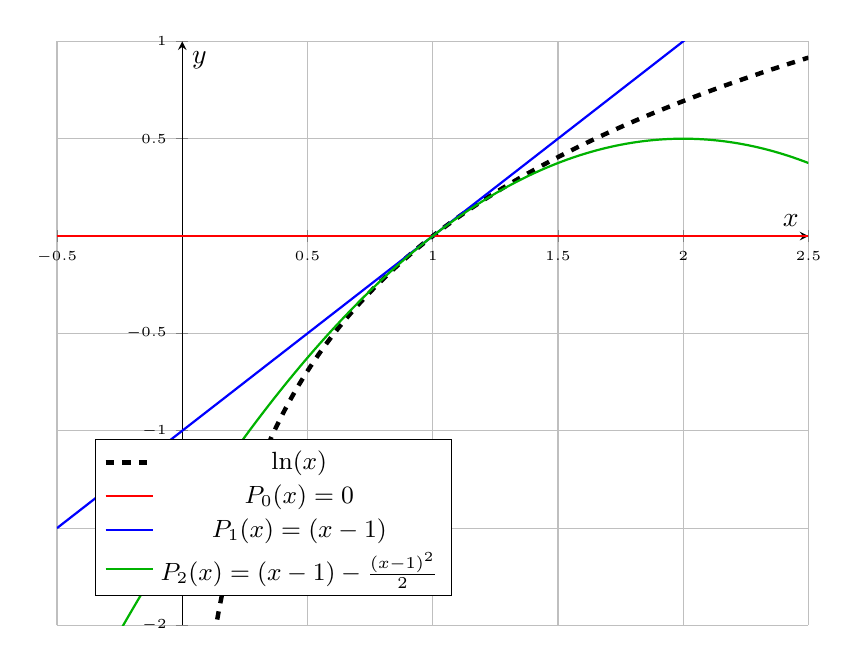
\begin{tikzpicture}
    \begin{axis}[
        xlabel={$x$},
        ylabel={$y$},
        xmin=-0.5, xmax=2.5,
        ymin=-2, ymax=1,
        axis lines=middle,
        legend style={at={(0.05,0.05)}, anchor=south west, font=\small},
        grid=major,
        samples=150,
        domain=0.01:2.5,
        height=9cm,
        width=\linewidth-1cm,
        tick label style={font=\tiny}
    ]
    
    \addplot[black, dashed, ultra thick] {ln(x)};
    \addlegendentry{$\ln(x)$}

    \addplot[red, thick, domain=-0.5:2.5] {0};
    \addlegendentry{$P_0(x)=0$}

    \addplot[blue, thick, domain=-0.5:2.5] {x-1};
    \addlegendentry{$P_1(x)=(x-1)$}

    \addplot[green!70!black, thick, domain=-0.5:2.5] {(x-1) - 0.5*(x-1)^2};
    \addlegendentry{$P_2(x)=(x-1)-\frac{(x-1)^2}{2}$}

    \end{axis}
\end{tikzpicture}
\par\small\textit{Approximation de $\ln(x)$ autour de $a=1$. Le polynôme "colle" à la fonction près de $x=1$.}
\end{intuitionbox}


\subsection{La Fonction Exponentielle ($e^x$)}

\begin{theorembox}[Série de Maclaurin pour $e^x$]
Pour tout nombre réel $x$, la fonction exponentielle peut s'écrire :
$$ e^x = \sum_{k=0}^{\infty} \frac{x^k}{k!} = 1 + x + \frac{x^2}{2!} + \frac{x^3}{3!} + \frac{x^4}{4!} + \cdots $$
\end{theorembox}

\begin{intuitionbox}[Visualiser la Croissance Exponentielle]
La fonction exponentielle est unique car elle est sa propre dérivée. Cela signifie que toutes ses informations locales (valeur, pente, courbure) en $a=0$ sont égales à \textbf{1}. La série pour $e^x$ est donc le polynôme le plus « pur », où chaque terme $x^k$ est simplement normalisé par $k!$. Le graphique ci-dessous montre comment les polynômes de Taylor convergent rapidement vers la véritable courbe exponentielle, illustrant sa croissance puissante.

\tcblower

\centering
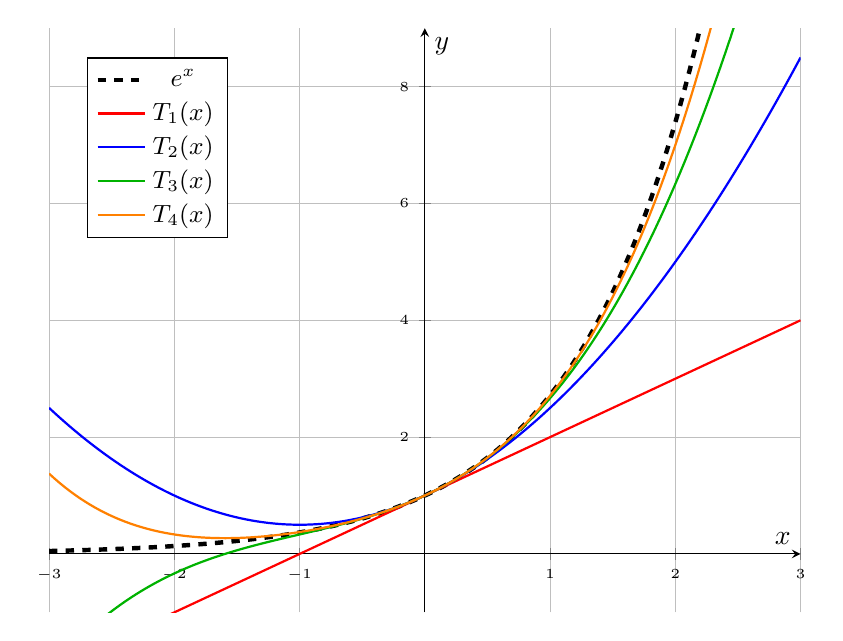
\begin{tikzpicture}
    \begin{axis}[
        xlabel={$x$},
        ylabel={$y$},
        xmin=-3, xmax=3,
        ymin=-1, ymax=9,
        axis lines=middle,
        legend style={at={(0.05,0.95)}, anchor=north west, font=\small},
        grid=major,
        samples=150,
        domain=-3:3,
        height=9cm,
        width=\linewidth-1cm,
        tick label style={font=\tiny}
    ]
    
    \addplot[black, dashed, ultra thick] {exp(x)};
    \addlegendentry{$e^x$}

    \addplot[red, thick] {1+x};
    \addlegendentry{$T_1(x)$}

    \addplot[blue, thick] {1+x+x^2/2};
    \addlegendentry{$T_2(x)$}

    \addplot[green!70!black, thick] {1+x+x^2/2+x^3/6};
    \addlegendentry{$T_3(x)$}

    \addplot[orange, thick] {1+x+x^2/2+x^3/6+x^4/24};
    \addlegendentry{$T_4(x)$}

    \end{axis}
\end{tikzpicture}
\par\small\textit{Approximation de $e^x$ par ses polynômes de Maclaurin.}
\end{intuitionbox}

\begin{proofbox}
Soit $f(x) = e^x$. Pour tout entier $k \ge 0$, la $k$-ième dérivée est $f^{(k)}(x) = e^x$. En évaluant en $a=0$, on obtient $f^{(k)}(0) = e^0 = 1$ pour tout $k$. En appliquant la formule de Maclaurin :
$$ e^x = \sum_{k=0}^{\infty} \frac{f^{(k)}(0)}{k!} x^k = \sum_{k=0}^{\infty} \frac{1}{k!} x^k = 1 + x + \frac{x^2}{2} + \frac{x^3}{6} + \cdots $$
\end{proofbox}


\subsection{La Fonction Sinus ($\sin(x)$)}

\begin{theorembox}[Série de Maclaurin pour $\sin(x)$]
Pour tout nombre réel $x$ :
$$ \sin(x) = \sum_{k=0}^{\infty} (-1)^k \frac{x^{2k+1}}{(2k+1)!} = x - \frac{x^3}{3!} + \frac{x^5}{5!} - \frac{x^7}{7!} + \cdots $$
\end{theorembox}

\begin{intuitionbox}[Visualiser l'Oscillation du Sinus]
La série du sinus reflète ses propriétés fondamentales. En tant que fonction \textbf{impaire} ($ \sin(-x) = -\sin(x) $), son développement ne contient que des puissances \textbf{impaires} de $x$. Les signes alternés capturent sa nature oscillatoire. Le graphique ci-dessous montre comment l'ajout de termes permet au polynôme d'« épouser » la courbe du sinus sur un plus grand nombre de périodes.

\tcblower

\centering
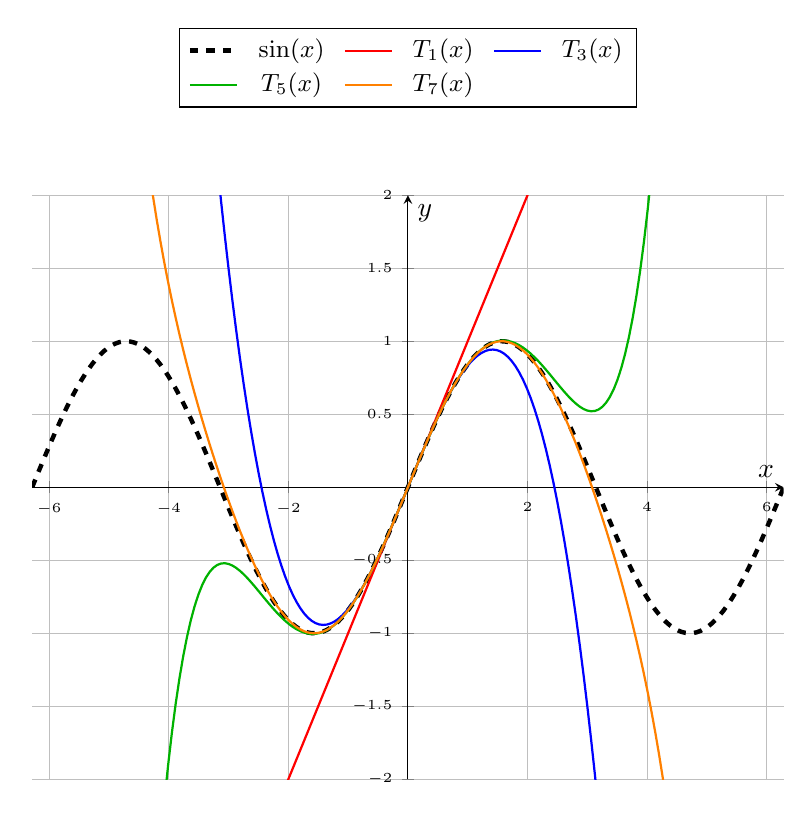
\begin{tikzpicture}
    \begin{axis}[
        xlabel={$x$},
        ylabel={$y$},
        xmin=-2*pi, xmax=2*pi,
        ymin=-2.0, ymax=2.0,
        axis lines=middle,
        legend style={at={(0.5,1.15)}, anchor=south, font=\small, column sep=5pt},
        legend columns=3,
        grid=major,
        samples=200,
        domain=-2*pi:2*pi,
        height=9cm,
        width=\linewidth-1cm,
        tick label style={font=\tiny}
    ]
    \addplot[black, dashed, ultra thick] {sin(deg(x))};
    \addlegendentry{$\sin(x)$}
    \addplot[red, thick] {x};
    \addlegendentry{$T_1(x)$}
    \addplot[blue, thick] {x - (x^3)/6};
    \addlegendentry{$T_3(x)$}
    \addplot[green!70!black, thick] {x - (x^3)/6 + (x^5)/120};
    \addlegendentry{$T_5(x)$}
    \addplot[orange, thick] {x - (x^3)/6 + (x^5)/120 - (x^7)/5040};
    \addlegendentry{$T_7(x)$}
    \end{axis}
\end{tikzpicture}
\par\small\textit{Approximation de $\sin(x)$ par ses polynômes de Maclaurin.}
\end{intuitionbox}

\begin{proofbox}
Soit $f(x) = \sin(x)$. Les dérivées en $a=0$ suivent un cycle $(0, 1, 0, -1, \dots)$. Seuls les termes d'ordre impair ($2k+1$) sont non nuls, avec des valeurs de $(-1)^k$, ce qui donne la formule.
\end{proofbox}


\subsection{La Fonction Cosinus ($\cos(x)$)}

\begin{theorembox}[Série de Maclaurin pour $\cos(x)$]
Pour tout nombre réel $x$ :
$$ \cos(x) = \sum_{k=0}^{\infty} (-1)^k \frac{x^{2k}}{(2k)!} = 1 - \frac{x^2}{2!} + \frac{x^4}{4!} - \frac{x^6}{6!} + \cdots $$
\end{theorembox}

\begin{intuitionbox}[Visualiser la Symétrie du Cosinus]
En tant que fonction \textbf{paire} ($ \cos(-x) = \cos(x) $), la série du cosinus ne contient, de manière appropriée, que des puissances \textbf{paires} de $x$. Elle commence à 1 (son maximum) puis oscille, un comportement capturé par les signes alternés.

\tcblower

\centering
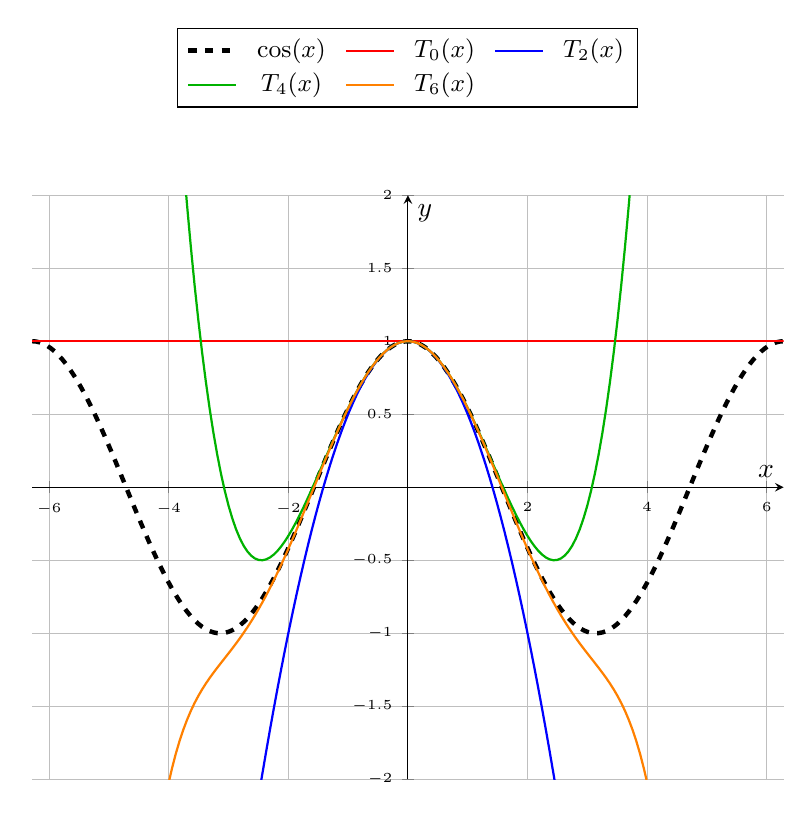
\begin{tikzpicture}
    \begin{axis}[
        xlabel={$x$},
        ylabel={$y$},
        xmin=-2*pi, xmax=2*pi,
        ymin=-2.0, ymax=2.0,
        axis lines=middle,
        legend style={at={(0.5,1.15)}, anchor=south, font=\small, column sep=5pt},
        legend columns=3,
        grid=major,
        samples=200,
        domain=-2*pi:2*pi,
        height=9cm,
        width=\linewidth-1cm,
        tick label style={font=\tiny}
    ]
    \addplot[black, dashed, ultra thick] {cos(deg(x))};
    \addlegendentry{$\cos(x)$}
    \addplot[red, thick] {1};
    \addlegendentry{$T_0(x)$}
    \addplot[blue, thick] {1 - x^2/2};
    \addlegendentry{$T_2(x)$}
    \addplot[green!70!black, thick] {1 - x^2/2 + x^4/24};
    \addlegendentry{$T_4(x)$}
    \addplot[orange, thick] {1 - x^2/2 + x^4/24 - x^6/720};
    \addlegendentry{$T_6(x)$}
    \end{axis}
\end{tikzpicture}
\par\small\textit{Approximation de $\cos(x)$ par ses polynômes de Maclaurin.}
\end{intuitionbox}

\begin{proofbox}
Soit $g(x) = \cos(x)$. Les dérivées en $a=0$ suivent un cycle $(1, 0, -1, 0, \dots)$. Seuls les termes d'ordre pair ($2k$) sont non nuls, avec des valeurs de $(-1)^k$, ce qui donne la formule.
\end{proofbox}


\subsection{Le Logarithme Népérien ($\ln(1+x)$)}

\begin{theorembox}[Série de Maclaurin pour $\ln(1+x)$]
Pour $|x| < 1$ :
$$ \ln(1+x) = \sum_{k=1}^{\infty} (-1)^{k-1} \frac{x^k}{k} = x - \frac{x^2}{2} + \frac{x^3}{3} - \frac{x^4}{4} + \cdots $$
\end{theorembox}

\begin{intuitionbox}[Visualiser l'Approximation Logarithmique]
Cette série est essentielle pour approximer les logarithmes près de 1. Contrairement aux fonctions précédentes, elle ne converge que pour $|x|<1$. Le graphique montre que l'approximation est excellente près de $x=0$ mais diverge rapidement lorsque $x$ s'approche de la frontière de convergence à $x=1$.

\tcblower

\centering
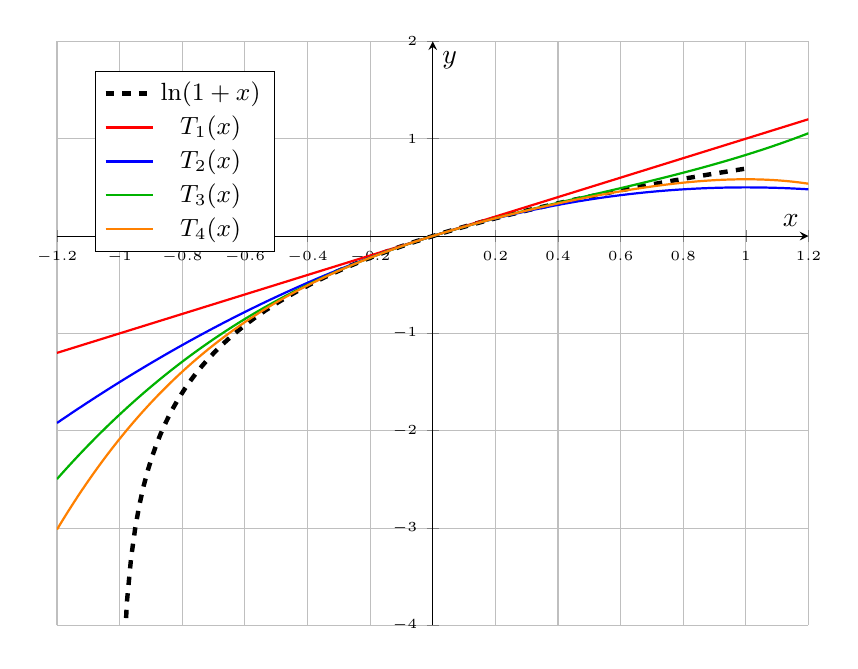
\begin{tikzpicture}
    \begin{axis}[
        xlabel={$x$},
        ylabel={$y$},
        xmin=-1.2, xmax=1.2,
        ymin=-4, ymax=2,
        axis lines=middle,
        legend style={at={(0.05,0.95)}, anchor=north west, font=\small},
        grid=major,
        samples=150,
        domain=-0.99:1, % Domain restricted for ln
        height=9cm,
        width=\linewidth-1cm,
        tick label style={font=\tiny}
    ]
    \addplot[black, dashed, ultra thick] {ln(1+x)};
    \addlegendentry{$\ln(1+x)$}
    
    \addplot[red, thick, domain=-1.2:1.2] {x};
    \addlegendentry{$T_1(x)$}

    \addplot[blue, thick, domain=-1.2:1.2] {x - x^2/2};
    \addlegendentry{$T_2(x)$}

    \addplot[green!70!black, thick, domain=-1.2:1.2] {x - x^2/2 + x^3/3};
    \addlegendentry{$T_3(x)$}
    
    \addplot[orange, thick, domain=-1.2:1.2] {x - x^2/2 + x^3/3 - x^4/4};
    \addlegendentry{$T_4(x)$}

    \end{axis}
\end{tikzpicture}
\par\small\textit{Approximation de $\ln(1+x)$ par ses polynômes de Maclaurin.}
\end{intuitionbox}

\begin{proofbox}
Soit $f(x) = \ln(1+x)$. Pour $k \ge 1$, la $k$-ième dérivée en $a=0$ est $f^{(k)}(0) = (-1)^{k-1} (k-1)!$. En substituant cela dans la formule de Maclaurin, le $(k-1)!$ au numérateur annule partiellement le $k!$ au dénominateur, laissant un $k$ en bas.
\end{proofbox}

\subsection{La Série Géométrique ($\frac{1}{1-x}$)}

\begin{theorembox}[Série de Maclaurin pour $\frac{1}{1-x}$]
Pour $|x| < 1$ :
$$ \frac{1}{1-x} = \sum_{k=0}^{\infty} x^k = 1 + x + x^2 + x^3 + \cdots $$
\end{theorembox}

\begin{intuitionbox}[Le Fondement de Nombreuses Séries]
Cette série, connue sous le nom de série géométrique, est l'un des développements en série de puissances les plus fondamentaux. Elle converge uniquement lorsque la valeur absolue de $x$ est inférieure à 1. Chaque coefficient est simplement 1, ce qui en fait la série de Maclaurin la plus simple. De nombreuses autres séries, comme celle de $\ln(1+x)$ ou de $\arctan(x)$, peuvent être dérivées de celle-ci par intégration ou substitution.
\end{intuitionbox}

\begin{proofbox}
Soit $f(x) = (1-x)^{-1}$. Les dérivées successives sont $f'(x) = 1(1-x)^{-2}$, $f''(x) = 2(1-x)^{-3}$, $f'''(x) = 6(1-x)^{-4}$, et ainsi de suite. La formule générale pour la $k$-ième dérivée est $f^{(k)}(x) = k!(1-x)^{-(k+1)}$. En évaluant en $a=0$, on obtient $f^{(k)}(0) = k!$. En substituant dans la formule de Maclaurin :
$$ \frac{1}{1-x} = \sum_{k=0}^{\infty} \frac{f^{(k)}(0)}{k!} x^k = \sum_{k=0}^{\infty} \frac{k!}{k!} x^k = \sum_{k=0}^{\infty} x^k $$
\end{proofbox}